\documentclass[../thesis.tex]{subfiles}

\begin{document}

  \chapter{Experimental results}
  \label{ch:experimental-results}


    \section{Experimental approach}
    \label{sec:conducted-measurements}

        For the first time during the team's research on alumina membranes, systematic measurements were conducted. Due to the limited period of time, only some aspects of the membranes could be investigated in more detail. During the internship, I measured 25 membranes of 3 wafers using the experimental setup described in \cref{sec:experimental-setup}. \Cref{tbl:wafer-specifications} summarizes the main fefatures of these wafers.

        \subfile{tikz/wafers/membrane_distribution.tex}

        \begin{table}[tb]
          \caption{Wafer specifications. The wafers thickness $l_\mathrm{pore}$, floating time $t_\mathrm{float}$ of the \textit{barrier layer} dissolution process and pore diameter dispersion $\Delta d_\mathrm{pore}^\mathrm{MEB}$ measured by electron beam microscopy are noted. The latter two parameters apply to the open pore membranes of the respective wafer.}
          \label{tbl:wafer-specifications}
          \selectfontsize{10pt}
          \begin{tabu} {X[r]X[r]X[r]X[r]}
            \unitoprule \\
            \textbf{Wafer} & \textbf{$l_\mathrm{pore}$ $[\si{\micro\meter}]$} & \textbf{$t_\mathrm{float}$ $[\si{\minute}]$} & \textbf{$\Delta d_\mathrm{pore}^\mathrm{MEB}$ $[\si{\nano\meter}]$} \\
            \unimidrule \\
            292 &60  &36+4   &- \\
            294 &60  &33   &-  \\
            295 &30  &35 (38 for b)  &7  \\
            296 &60  &40  &-  \\
            \unitoprule \\
          \end{tabu}
        \end{table}
        \medskip

        Victor Doebele's inital measurements previous to this internship had already shown strong dispersions in the properties of the membranes of different wafers, but also within the same wafer. Therefore, my goal was to perform systematic measurements on alumina membranes to determine the source of these dispersions. To probe a possible dependency on the position of the membranes on the wafers, the labeling is done according to the convention shown in \cref{fig:membrane-distribution}.

        Due to the limited period of time, I chose to focus on the production step of the \textit{barrier layer} dissolution (compare \cref{subsec:barrier-layer-dissolution}) and the pore diameter reduction by atomic layer deposition. During the intership, I measured 25 membranes of 4 wafers using the experimental setup described in \cref{sec:experimental-setup}. \Cref{tbl:wafer-specifications} summarizes the main characteristics of these wafers. A processing scheme for the wafers 295 and 296, which also marks the conducted measurements, is given by \cref{fig:wafer-processing-plans}.
        \medskip

        \subfile{tikz/wafers/wafer_processing_plans.tex}


    \section{Membrane structure analysis}

      \subsection{Isotherm of an open pore membrane}
      \label{subsec:open-pore-isotherm}

        \Cref{fig:295b-open-pores} shows a typical isotherm obtained from the measurements of an open pore membrane (in this case membrane 296b'). The dependence of the liquid fraction $LF$ on the relative vapor pressure $P_\mathrm{rel}$ follows the behaviour expected for a porous material: The membrane fills at a pressure
        \begin{equation*}
          P_\mathrm{cond}^\mathrm{296b'}<P_\mathrm{sv}
        \end{equation*}
        and empties at an even lower pressure
        \begin{equation*}
            P_\mathrm{evap}^\mathrm{296b'}<P_\mathrm{cond}^\mathrm{296b'}<P_\mathrm{sv},
        \end{equation*}
        hereby displaying a hysteretic cycle. By the model of condensation and evaporation in an open pore, which was introduced in \cref{eq:cond-evap-non-ideal-pore}, a condensation at spinodal pressure $P_\mathrm{sp}$ and evaporation at equilibrium pressure $P_\mathrm{eq}$, with
        \begin{equation*}
          P_\mathrm{eq}<P_\mathrm{sp}<P_\mathrm{sv},
        \end{equation*}
        are expected. This is coherent with the observations as the shape of the volumetric isotherm qualitatively matches the theoretical loop displayed in \cref{fig:open-pore-loops}. Other experimentators have made the same observations (compare \cite{Casanova2008a,Bruschi2015a}).

        For the tranmission measurement, two drops corresponding to the condensation and the evaporation are observed, as expected according to \cref{sec:scattering-in-alumina-membranes}. Moreover, higher transmission is observed for the filled state of the membrane than for the empty state. This is also coherent with the theory of index matching mentioned in \cref{sec:scattering-in-alumina-membranes}.
        \medskip

        The dashed lines in \cref{fig:295b-open-pores} mark the average condensation and evaporation pressures of the isotherm. For their determination, the steepest point of the liquid fraction graph is sought, which corresponds to the minima of the transmission signals as expected. Converting these to diameters using the \textsc{Kelvin} equations \cref{eq:p-sp} and \cref{eq:p-eq} yields
        \begin{align*}
          d_\mathrm{pore}^\mathrm{296b'}(P_\mathrm{rel,sp}^\mathrm{296b'}=0,956)=\SI{44,4}{\nano\meter}, \\
          d_\mathrm{pore}^\mathrm{296b'}(P_\mathrm{rel,eq}^\mathrm{296b'}=0,925)=\SI{51,3}{\nano\meter},
        \end{align*}
        which makes for results within the range of expeceted pore diameters. Furthermore, the transmission behaves according to theory in regard of the filled transmission in filled state being stronger than for the empty state.
        \medskip

        \subfile{tikz/graphs/open_pore/296b_op.tex}

        \begin{figure}[p]
          \centering
          \subfloat[]{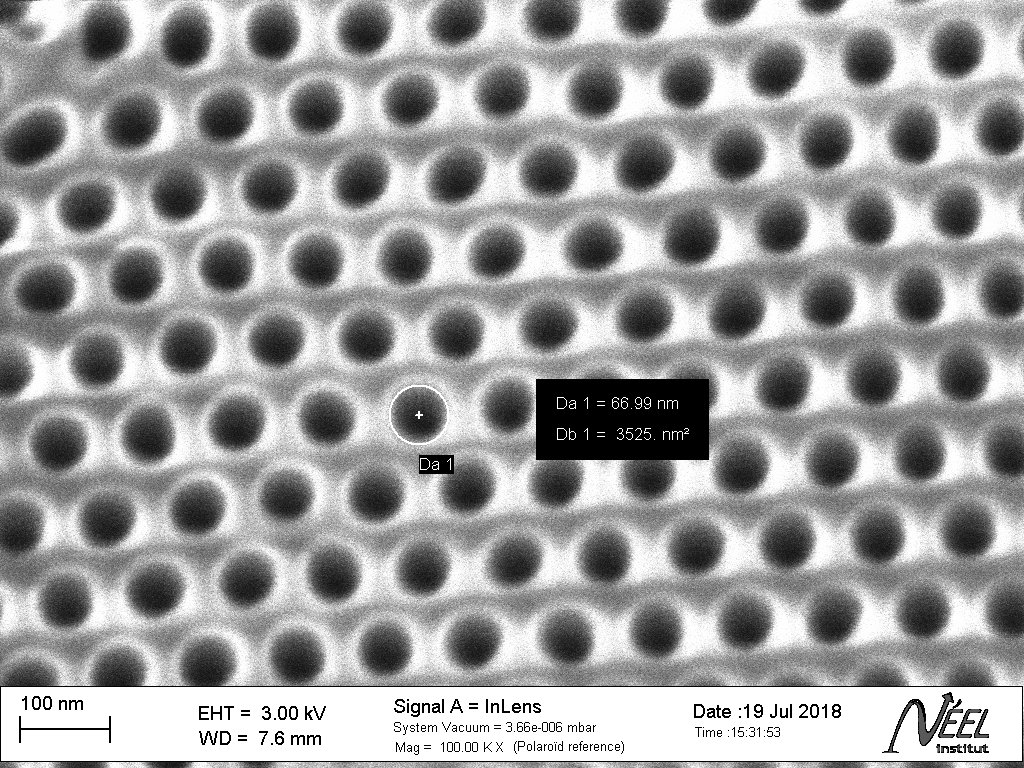
\includegraphics[width=.9\textwidth]{images/295g_pores_sol_side.jpg}
          \label{fig:295g-sol-side-sem}}
          \\
          \subfloat[]{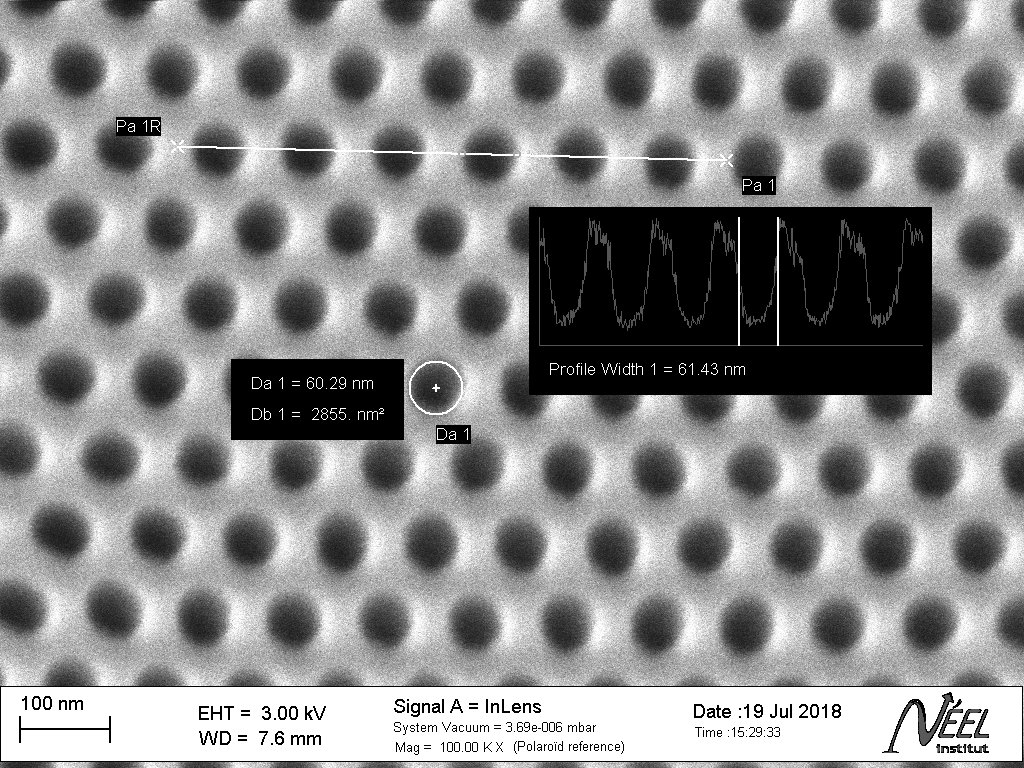
\includegraphics[width=.9\textwidth]{images/295g_pores_al_side.jpg}
          \label{fig:295g-al-side-sem}}
          \caption{SEM images of membrane 295g' implying the pores' funnellization. The pores on the solution side \protect\subref{fig:295g-sol-side-sem} show bigger diameters than those on the aluminum side \protect\subref{fig:295g-al-side-sem}.}
          \label{fig:295g-sem-funnellization-proof}
        \end{figure}

        However, if all the pores were cylindrical, the condensation and evaporation branches would be expected to be vertical. The inclination of evaporation branch could result from funnellization of the pores as has been explained in \cref{subsec:open-funnelled-pore-theory}. The SEM images of the membranes support the assumption of funnelled pores as different pore diameters are observed for the top and  bottom side (please refer to \cref{fig:295g-sem-funnellization-proof} for an example).  The condensation at spinodal pressure should still be vertical for weak funnelled pores, though. On the other hand, condensation at spinodal pressure in weakly funnelled cylindrical pores (compare \cref{subsec:open-funnelled-pore-theory}). This leads to the conclusion, that the pores are not only funnelled, but also distributed in diameter.



    \subsection{Isotherm of a closed pore membrane}
    \label{subsec:closed-pore-isotherm}

        \subfile{tikz/graphs/closed_pore_isotherm/cp_isotherm.tex}

        \Cref{fig:295b-closed-pores} shows the isotherm obtained on the same membrane 296b, but prior to the \textit{barrier layer} dissolution step. The open pore membrane's isotherm is also displayed for the sake of comparison. The results show that the hysteresis cycle is much smaller for closed pores than it has been observed for open pores. In detail, the condensation branch is shifted to much lower pressures, while the evaporation branch shows only a slight shift in the same direction.

        As will be explained in \cref{sec:opening-problem}, a small shift to lower pressures for the closed pore membrane is expected due to the widening of the pores during the \textit{barrier layer} dissolution process. Since, according to \cref{subsec:closed-funnelled-pore-theory}, the condensation occurs at equilibrium pressure in a closed pore, the smaller hysteresis of membrane 296b in comparison to 296b' is expected. However, as displayed in \cref{fig:closed-pore-loops}, the volumetric isotherm of a closed pore membrane should not show a hysteresis at all, not for straight pores and neither for funnelled pores. Its presence can be explained by variations of the pore diameters along the pores' lengths. These variations are so called \textit{corrugations}. The phenomenom of the hysteresis appearing for closed pores has been observed and accounted to corrugations by various experimentators (\cite{Mistura2016a,Morishige2016}) and \textsc{Monte Carlo} simulations that confirm the appearing hysteresis run by Joel Puibasset \cite{Puibasset2007a}.
        \medskip

        As for the transmission, the drops correspond to the condensation and evporation branch and also the effect of index matching is observed as expected from \cref{sec:scattering-in-alumina-membranes}. What remains to be understood is the extreme difference in magnitude between the transmission drops of the closed pore and the open pore membrane. In this magnitude, the phenomenom has only been observed for this specific membrane 296b so it might also be due to a light source within the experimental room that has not been turned off. As the membrane has been further processed, the measurement cannot be repeated though.


    \subsection{Measurement reproducibility}
    \label{subsec:measurement-reproducibility}

        \subfile{tikz/graphs/292c/292c_repro.tex}

        To check the reproducibility of the isotherm measurements, membranes were measured several times. \Cref{fig:292c-repro} shows four consecutive measurements for the same open pore membrane 292c and one more independent measurement ($LF_\mathrm{cond/evap}^\mathrm{292c,5}$). The biggest experiment deviation is the liquid fraction before the sharp rise of the condensation branch. However, this does not affect the position of the condensation and the evaporation rises, which are used to determine the pores' diameters.
        \medskip

        As at the time of these experiments the laser transmission setup had not been in place and later membranes were measured only two times at maximum, the reproducibility of the laser transmission measurements cannot be assesed here.


    \subsection{Inhomogeneities on one wafer}
    \label{subsec:wafer-inhomogeneities}

        \subfile{tikz/graphs/wafer_inhomogeneities/inhomogeneities_cp.tex}
        \subfile{tikz/graphs/wafer_inhomogeneities/inhomogeneities_op.tex}

        The homogeneity of several membranes on a wafer is importan for the planned helium experiments. When the aim of producing membranes with pores of diameters $d_\mathrm{pore}<\SI{10}{\nano\meter}$ is reached, the molar amount of hexane condensed within these pores becomes very small. Consequently, it becomes harder to detect a signal not only for the volumetric measurements, but due to the use of helium also for the transmission measurements. Therefore, stacks of several membranes might have to be used in the course of the experiments.
        \medskip

        In the following, the isotherm measurements I performed in order to test the homogeneity of the wafers are presented for two production steps: The closed pore state after the aluminum dissolution process (compare \cref{subsec:al-dissolution}) in \cref{fig:inhomogeneities-cp} and the open pores after the \textit{barrier layer} dissolution (\cref{subsec:barrier-layer-dissolution}) in\cref{fig:inhomogeneities-op}.

        For both wafers the overall shapes of the different membranes' isotherm measurements matches. The only exception is the open pore membrane 295c', which will be discussed in \cref{sec:theory-and-defects}. However, the results show that there is a dispersion on the condensation and evaporation branches. This implies a dispersion on the pore size distribution of about
        \begin{align*}
          \Delta d_\mathrm{closed-pore}^\mathrm{296} = \SI{3,5}{\nano\meter} \\
          \Delta d_\mathrm{closed-pore}^\mathrm{295} = \SI{4,7}{\nano\meter}
        \end{align*}
        for the closed pore membranes and
        \begin{align*}
          \Delta d_\mathrm{open-pore}^\mathrm{292} = \SI{4,1}{\nano\meter} \\
          \Delta d_\mathrm{open-pore}^\mathrm{295} = \SI{3,5}{\nano\meter}
        \end{align*}
        for the open pore membranes. The computations were done using the pressures of the top end of the widest spread evaporation branches of the respective wafer
        \begin{align*}
          P_\mathrm{evap,top}^\mathrm{296b}=0,9275,\quad P_\mathrm{evap,top}^\mathrm{296e'}=0,9225, \\
          P_\mathrm{evap,top}^\mathrm{295a}=0,9375,\quad P_\mathrm{evap,top}^\mathrm{295b}=0,9325, \\
          P_\mathrm{evap,top}^\mathrm{292c}=0,9275,\quad P_\mathrm{evap,top}^\mathrm{292d}=0,9325, \\
          P_\mathrm{evap,top}^\mathrm{295d'}=0,9430,\quad P_\mathrm{evap,top}^\mathrm{295e'}=0,9400,
        \end{align*}
        as these correspond to the emptying of the largest pores of a given membrane.
        \medskip

        Moreover, the transmission during the condensation and the evpoatiion of hexane within the membranes also shows dispersions across the wafers. \Cref{fig:wafer-transmission} shows color maps of the dry transmission of the membranes of the wafers 295 and 296. The membranes of wafer 296 have all been measured before any further treatments with phosphoric acid, whereas the membranes of wafer 295 are open pore membranes except for 295a and 295b, which are still closed. In comparison to the theoretical values computed using the \textsc{Fresnel} equations (compare \cref{eq:trans-coeffs}), the measured transmission coefficients are much smaller. This can be explained by the pores scattering light as explained in \cref{sec:scattering-in-alumina-membranes}. Talking wafer inhomogeneities, the measured transmission of membranes on the same wafer shows variations of up to $\SI{8}{\percent}$
        for the closed pore membrane of wafer 296 and $\SI{17}{\percent}$ for the open pore membranes of 295. A systematics regarding the the link between the pore diameters and the transmission value can be suspected when regarding the membranes 296a, 296b, 296e and 296f. For each pair of two neighboring membranes, the same transmission has been measured. The respective isotherms are displayed in \cref{fig:296-cp}. What strikes the eye is that the neighboring pores show almost perfectly superimposed volumetric isotherms, whereas the there is a clear shift in pressure between the two pairs' curves. To draw a conclusion, larger pore diameters (higher condensation pressures) go together with a stronger dry transmission. This conclusion has to be retested using other membranes as it has only been observed once.

        \subfile{tikz/wafers/transmission.tex}

        In conclusion, to measure the effect of treatments on a given membrane, before and after measurements are necessary. It is not enough to measure one membrane representatively for multiple membranes in the same state.


        \subsubsection{Stronger light scattering for larger pore diameters?}

          \Cref{fig:295-transmission} shows the measured dry transmission for the membranes of wafer 295. The membranes 295a and 295b are still closed pore membranes, while all other membranes have undergone the \textit{barrier layer} dissolution process opening their pores. Striking is the much better transmission of the closed pore membranes in comparison to the open pore membranes. Referring to the assumption made in \cref{subsec:wafer-inhomogeneities}, that larger pores cause stronger light scattering and therefore weaker transmission, the observed phenomenom could be explained by the increase of pore diameters upon the pore opening step. To verify this explanation, systematic experiments using the same open pore membrane and widening the pores by immersion in acid could be conducted.


        \subsubsection{The aluminum dissolution step affects the pores}
        \label{sssec:al-diss-bath}

          The wafer inhomogeneities appear after the step of the aluminum dissolution process already. In the interest of locating the origin of the dispersions of the wafers, the aluminum dissolution process has been probed even though by theory, the alumina should not be attacked by the used acid (compare \cref{subsec:al-dissolution}). To either confirm or refute the assumption that the process does not affect the pores, membrane 295a has been immersed in the same acid that is also used for the aluminum dissolution for $\SI{4,5}{\hour}$, the acid's temperature is $\SI{0}{\celsius}$, same as for the production step. For the aluminum dissolution, the wafers are immersed for about $\SI{4}{\hour}$, so any observation made on this experiment should be comparable to what happens during the production step.
          \medskip

          \Cref{fig:295a-al-diss} shows the comparison of the membrane 295a before the bath in the acid used for the aluminum dissolution and the membrane 295a' after the bath. While the shape of the isotherms does not change, a slight shift towards higher pressures and respectively higher diameters is observable. In conclusion, the acid does not only attack aluminum, but also alumina. If this process causes any pore defects like corrugations or funnellization is unclear. This should be probed by experimenting with several membranes and different immersion times in the acid.

          \subfile{tikz/graphs/295a_before_after_al_diss_bath/295a_before_after.tex}


    \subsection{Defects}
    \label{subsec:defects}

        The conducted measurements revealed defects and dispersions of the pores of one wafer and even one membrane. First, there is the pore size distribution. Next, the funnellization and the corrugation must be mentioned. Both cause intra pore diameter variations that cause inclined isotherms, even for a single pore. Last, bad open pores were detected during the measurements. This problem will be discussed in the following section, as its examination leads to valuable, relevant results.


  \section{The problem of pore opening}
  \label{sec:opening-problem}


      \subsection{Bad open pores}
      \label{subsec:bad-open-pores}

        \subfile{tikz/graphs/294_bad_open_pores/294_bad_open_pores.tex}

        Victor Doebele's measurements before my internship had revealed that the \textit{barrier layer} dissolution step failed to open all the pores of some membranes. The term \textit{bad open pores} refers to a membrane that has been floated on phosphoric acid for not long enough to completely open the pores. As a result some pores remain closed whereas others have constricted openings and some are fully open. \Cref{fig:294-bad-open-pores} shows the comparison of closed pore membrane 294cp and membrane 294op with bad open pores. The assumption of bad open opres is derived from the isotherm in the following way: By theory, the condensation branch should be shifted towards higher pressure for open pores in respect to closed pores. While this is the case for membrane 294op's end of the condensation rise, it still starts at the same pressure as the condensation of the closed pore membrane which by theory condenses at equilibrium pressure. Moreover, the evaporation of 294op is superimposed with the one of 294cp. While this is expected by theory, it rules out the possibility of an increase in funnellization or corrugation causing the broader condensation branch of the open pore membrane. The only possible explanation for the observed behaviour is a population of open pores alongside one of closed pores on the membrane. In this case some pores start filling at equilibrium pressure, wheras others fill at higher spinodal pressures depending on the size of the pore opening on the aluminum side. Independently, SEM images of the membrane confirm the assumption of bad open pores as shown in \cref{fig:294-sem}.

        \begin{figure}[p]
          \centering
          \subfloat[]{
          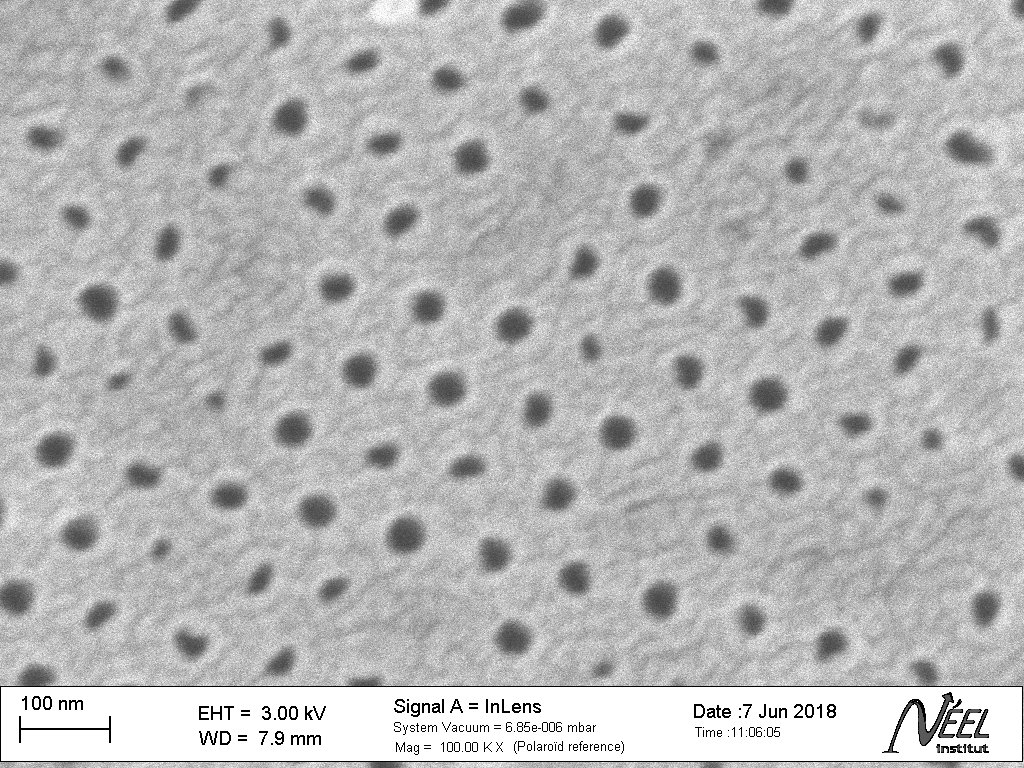
\includegraphics[width=0.9\textwidth]{images/294_bad_open_pores.jpg}
          \label{fig:294-sem}}  \\
          \subfloat[]{
          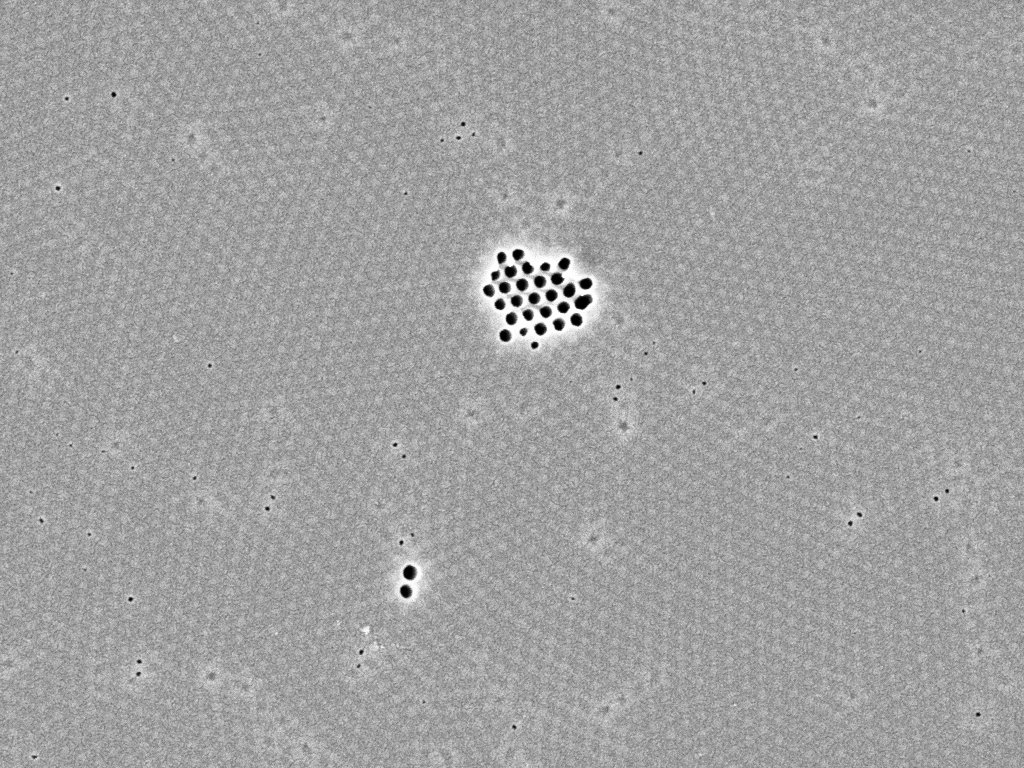
\includegraphics[width=0.9\textwidth]{images/sem_milky_etch.jpg}
          \label{fig:milky-meb}}
          \caption{\protect\subref{fig:294-sem} shows a SEM image confirming the bad open pores of membrane 294op. Image \protect\subref{fig:milky-meb} SEM image of a membran floated on phosphoric acid until the appearance of milky aspects. It is coherent with the link of the milky aspect to pores of a wafer starting to open.}
        \end{figure}

        At first glance, resolving the bad open pore issue seems as easy as simply increasing the membranes' floating time during the \textit{barrier layer} dissolution. On second thought though, a problem comes up: \Cref{fig:294-sem} clearly states that some pores open before others. Therefore, these open pores are infiltrated by phosphoric acid which starts etching the pore from the inside increasing its diameter. This results in a broadening pore diameter distribution on the membrane caused by the \textit{barrier layer} dissolution process.

        As mentioned in \cref{subsec:barrier-layer-dissolution}, milky aspects occur at some point of the floating. Same as for spinodal condensation in the membranes, the filling of the opening pores with acid is assumed to cause light scattering and can therfore be linked to these milky aspects. Proof of this theory is the SEM image taken of a membrane that has been floated until the milky aspects appeared. Shown in \cref{fig:milky-meb}, the image confirms the semi open state of the membrane. As the milky aspects last for about
        \begin{equation*}
          t_\mathrm{milky} =\SI{3}{\minute}
        \end{equation*}
        and the etch rate of phosphoric acid on alumina is expected to be
        \begin{equation*}
          e=\SI{1}{\nano\meter\per\second},
        \end{equation*}
        the \text{barrier layer} dissolution process should cause an increase of the pore diameter dispersion of
        \begin{equation*}
          \Delta d_\mathrm{pore} = \SI{6}{\nano\meter}.
        \end{equation*}
        This is quite dramatic regarding that the pore diameter distribution of a closed pore limited to about $\SI{10}{\nano\meter}$ (assuming the steepness of the evaporation branch only depends on the pore diameter distribution). Therefore, this increase should be obvious on the comparison of the evaporation branches of a closed pore membrane with an equivalent open pore membrane. Using \cref{fig:295b-closed-pores} as an example does not confirm these expectations. On the contrary, the evaporation branch seems to become more sharp by opening the pores. This leads to the suspicion that the etch rates parallel to the pore axis $e_\mathrm{\parallel pores}$ and perpendicular to the axis $e_\mathrm{\perp pores}$ are different. With the idea of using a combination of floating and immersion in phosphoric acid for the \textit{barrier layer} dissolution, an experiment to calibrate the etch rates has been conducted.
        \medskip

        Membranes of wafer 296 were floated and immersed in phosphoric acid for
        \begin{align*}
            \begin{split}
                t_\mathrm{im}^\mathrm{296c'}=\SI{6,5}{\minute}, \\
                t_\mathrm{im}^\mathrm{296d'}=\SI{13}{\minute},  \\
                t_\mathrm{fl}^\mathrm{296e'}=\SI{13}{\minute}, \\
                t_\mathrm{fl}^\mathrm{296f'}=\SI{26}{\minute},
            \end{split}
        \end{align*}
        where $t_\mathrm{im}^{i}$ are the immersion times and $t_\mathrm{fl}^{i}$ the floating times with $i\in \{ \mathrm{296c,296d,296e,296f}\}$. Assuming that the acid etches the \textit{barrier layer} at the same rate from within and outside the pores, these floating and immersion of the membranes 296c' and 296e' should yield the same reduction of the thickness, the same holds for the membranes 296d' and 296f'. At this point, the initial thickness of wafer 296 is assumed to be
        \begin{equation*}
          d_\mathrm{barrier-layer}^\mathrm{296} =\SI{30}{\nano\meter}
        \end{equation*}
        thick, same as for wafer 292. To probe the etch rate $e_\parallel$, SEM images are taken for all membranes after the treatment in phosphoric acid. These images also serve to measure the pore diameters on the solution side and hereby to calculate $e_\perp$. In addition, the pore diameters are checked using isotherm measurements.


        \subsection{Etch rate on the barrier layer}
        \label{subsec:etch-rate}

          \subfile{tikz/graphs/296_membranes/296_membranes.tex}

          \Cref{fig:barrier-layer-sems} shows the SEM images taken of the membranes 296c' and 296e' after immersion and floating respectively. During the SEM session, a lot of drift and charging had to be dealt with which makes for a bad resolution of the images. However, what strikes the eye is the large thickness of the \textit{barrier layer}, even after the treatments with phosphoric acid, as it is still thicker than the inital thickness that has been assumed. In accordance with these SEM images, the isotherm comparison shown in \cref{fig:full-comp-w296} implies pores that are still closed on all four treated membranes. In explanation, the isotherms superimpose nicely with the untreated closed pore membrane 296a and also, the direct comparison to the open pore membrane 296b' reveals a strong shift of the condensation branch towards lower pressures. Bad open pores can be excluded by comparing to \cref{fig:294-bad-open-pores} and the corresponding explanations in \cref{subsec:bad-open-pores}.

          In conclusion, the anodization process (compare \cref{subsec:anodizing} does not yield the same \textit{barrier layer} thickness for different wafers, even when the same parameters are used. The first thing to check is, if there is a dispersion of the \textit{barrier layer} thickness on one given wafer. Therefore, every other membrane (a, c, e, g, i, k) should be imaged using the SEM. Then, floating the remaining membranes for different periods of time and using the SEM again for imaging would yield a statisical value for the etch rate on the \textit{barrier layer}. To check if this etch rate can be assumed to be universal for all wafers, the process should be repeated for another wafer.

          \begin{figure}[p]
            \centering
            \subfloat[]{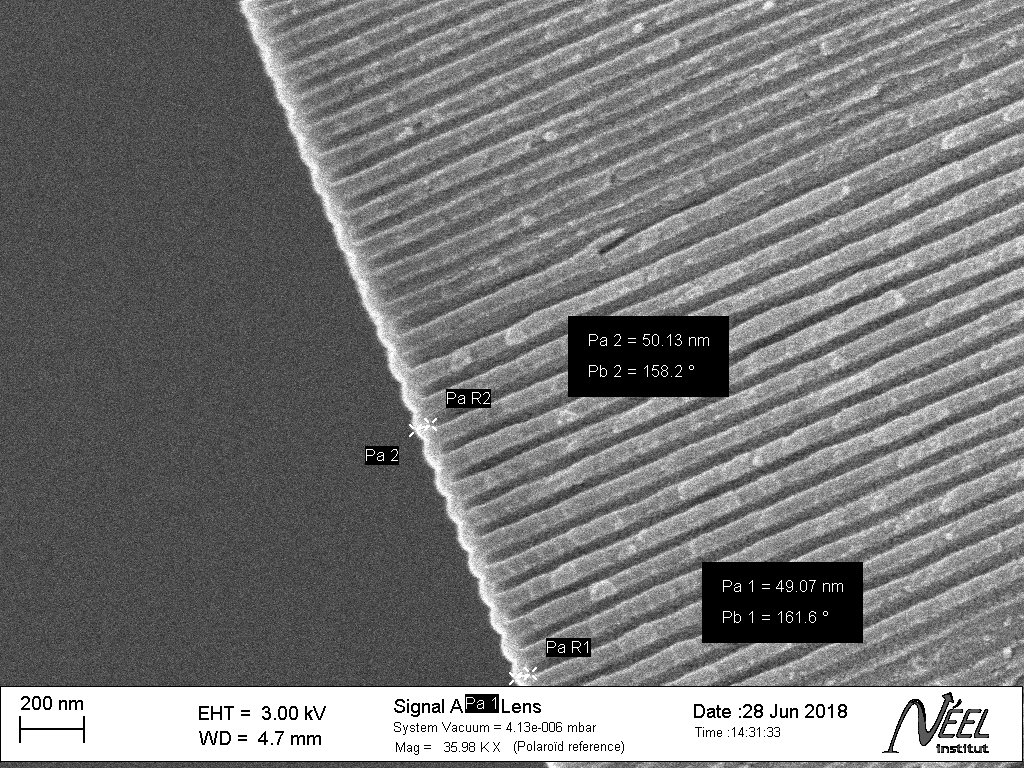
\includegraphics[width=0.9\textwidth]{images/296c_barrier_layer.jpg}
            \label{fig:296c-barrier-layer}} \\
            \subfloat[]{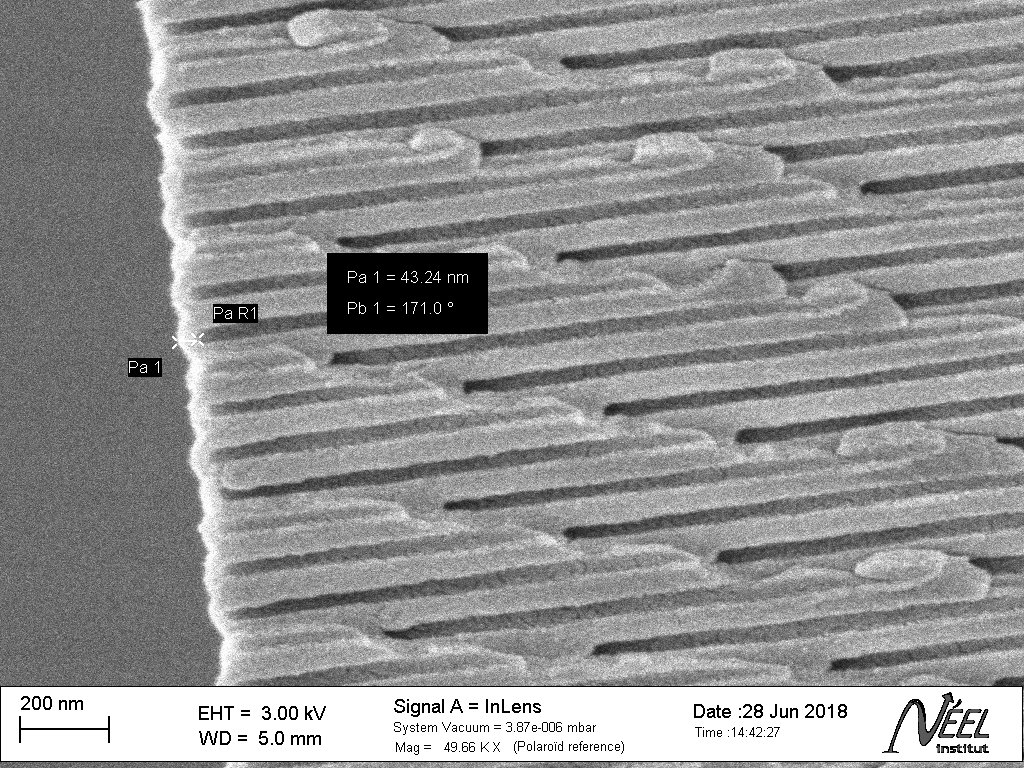
\includegraphics[width=0.9\textwidth]{images/296e_barrier_layer_meb.jpg}
            \label{fig:296e-barrier-layer}}
            \caption{SEM images with the aim to measure the thickness of the \textit{barrier layer} of the membranes 296c' and 296e'.}
            \label{fig:barrier-layer-sems}
          \end{figure}


        \subsection{Increase of funnellization upon immersion in phosphoric acid}
        \label{subsec:immersion-funnelling}

          \subfile{tikz/graphs/immersion_experiment/immersion.tex}

          The comparison of the immersed membranes 296c' and 296d' with the native membrane 296a yields a promising result. \Cref{fig:immersed-comp-w296} shows the three measured isotherms on a realtive vapor pressure axis revealing a shift of the top side of the evaporation rise to larger pressures going together with longer immersion times. At the same time, the bottom end of the condensation rise does not move to higher pressures. As it is closed pores that are dealt with (compare \cref{subsec:etch-rate}), the top end of the evaporation branch corresponds to the pore diameter at the top and, whereas the bottom end of the condensation branch corresponds to the diameter at the (smaller) closed end.
          \medskip

          Therefore, the observed phenomenom implies an etch rate that weakens along the pore axis towards the closed end. We speculate that this is due to saturation of the acid wihtin the pore as a result of the limited circulation.
          \medskip

          For further analysis of this acid saturation, \cref{fig:immersion-evap} and \cref{fig:immersion-cond} show \textsc{Kelvin} diameter conversions of the relevant pressure ranges. When converting $P_\mathrm{rel}$ to $d_\mathrm{pore}^\mathrm{Kelvin}$, the diameter offset increases linearly along the liquid fraction which corresponds to the position in along the pore axis of a funnelled pore (assuming that the isotherms' slopes only reflect funnellization). The etch rate gradient along the pore length as plotted in \cref{fig:etch-rate-plot} can be derived from the values noted in \cref{tbl:etch-rate}. The corresponding shape evolution of a pore is illustrated in \cref{fig:funneling-increase}.

          \begin{table}[tb]
           \caption{Diameter reduction per minute of immersion derived from the isotherms of the membranes 296a, 296c, 296d.}
           \label{tbl:etch-rate}
           \selectfontsize{10pt}
           \begin{tabu} {X[r]X[r]X[r]}
             \unitoprule \\
             \textbf{$t_\mathrm{im} [\si{\minute}]$} & \textbf{$\Delta d_{h=\SI{60}{\micro\meter}} [\si{\nano\meter}]$} & \textbf{$\Delta d_{h=\SI{0}{\micro\meter}} [\si{\nano\meter}]$} \\
             \unimidrule \\
             0 &0  &0 \\
             6,5 &3  &0  \\
             13  &6  &0  \\
             \unitoprule \\
           \end{tabu}
          \end{table}

          \subfile{tikz/wafer_analysis/funnelling_increase.tex}


        \subsection{Inverse funnellization upon barrier layer dissolution}
        \label{subsec:inverse-funnelling}

          With the results of the immersion experiment explained above in \cref{subsec:inverse-funnelling}, the comparison of closed and open pore isotherms can be further analysed. \Cref{fig:op-cp-comp} shows two plots. Both compare the isotherm measured for a given membrane in closed state to the isotherm measured for the \textit{same membrane} after the \textit{barrier layer} dissolution. This permits the comparison disregarding the intra wafer dispersions that were concluded in \cref{subsec:wafer-inhomogeneities}. The regarded membranes are 295b and 296b, respectively $\SI{30}{\micro\meter}$ and $\SI{60}{\micro\meter}$ thick.

          \subfile{tikz/graphs/cp_op_comp/cp_op_comp.tex}

          For both membranes, the isotherms steepen upon pore opening. Regarding the funnellization, the evaporation branch is of special interest. That it straightens upon the pore opening step implies that the funnellization decreases. Referring to the saturation of phosphoric acid within the pores upon immersion concluded in \cref{subsec:immersion-funnelling}, the inverse funnellization can be explained as follows: During the \textit{barrier layer} dissolution the pores begin to open when the milky aspects appear. When they have disappeared, one might think the pores are open. As explained in \cref{subsec:barrier-layer-dissolution}, the wafers are floated for $\SI{15}{\minute}$ more after the disappearance of the milky aspects to avoid bad opening observed on membrane 294op (compare \cref{subsec:bad-open-pores}).

          In conclusion, the phosphoric enters the pores from the small end saturates over at least $\SI{15}{\minute}$. During that time, the pores are straightened (inverse funnellization) as the etch rate is larger on the small ends of the pores.
          \medskip

          The attentive reader might have noticed the disappearance of the volumetric isotherm's kink of membrane 295b on the isotherm of open pore membrane 295b' that cannot be explained by the saturation of the acid. A possible interpretation of the occurence of this kink in the first place might be that the funnellization of the pores changes abruptly at a certain uniform position along the length of the pores (compare \cref{fig:weird-funnelling}). The reason for the correction of this defect upon the \textit{barrier layer} dissolution is not clear. One might speculate that it might be due to different etch rates of phosphoric acid on alumina that is contaminated by the chromatic acid used for the anodization of the wafers, and pure alumina (\cite{Rufolf-aam}). To check this possibility, the thickness and formation of the layer must be taken into account and further experiments conducted. Due to the limited period of time of my internship, this theory has not yet been further explored.
          \medskip

          However, another defect appears on the comparison of membrane 295b and 295b': The open pore membrane 295b' shows a two step condensation branch, whereas the evaporation happens at a single pressure. What strikes the eye is that the first rise of the condensation branch spreads on the same relative pressure range as the the evaporation branch. This raises the suspicion of pores filling at equilibrium pressure. Unlike the observations of bad open pore membrane 294op, the first rise of the condensation branch of membrane 295b' is followed by a plateau which leads to the next sharp rise. This implies two discreet pore populations of closed and open pores on the membrane, rather than bad open pores.

          \subfile{tikz/wafer_analysis/weird_pore_funnelling.tex}


  \section{Do thinner membranes improve things?}
  \label{sec:thinner-membranes}

    After having revealed the funnellization of the pores, the team had the idea to produce a wafer only half as thick as the old ones. Hereby, the effect of the funnellization on the isotherms should be reduced when assuming that the funnellization is linear throughout the pore. This idea resulted in the production of wafer 295, which is only
    \begin{equation}
        l^{295}_\mathrm{pore}=\SI{30}{\micro\meter}
    \end{equation}
    thick, whereas the previously produced and measured membranes had a thickness of
    \begin{equation}
        l^{292,293,294,296}_\mathrm{pore}=\SI{60}{\micro\meter}.
    \end{equation}

    \subfile{tikz/graphs/295_296_funnelling/295_296_funnelling.tex}

    \Cref{fig:295-296-funnelling-cp} shows the isotherms  of the membranes 295a and 296b on a \textsc{Kelvin} diameter axis. Both membranes' pores are closed by the \textit{barrier layer} on the bottom side. In contrast to expectations, the evaporation branches show a similar steepness that results in the a respective pore diameter difference between top and bottom end of
    \begin{align}
      \begin{split}
        \Delta d_\mathrm{evap}^\mathrm{295a}=\SI{15}{\nano\meter}, \\
        \Delta d_\mathrm{evap}^\mathrm{296b}=\SI{17}{\nano\meter},
      \end{split}
    \end{align}
    when assuming the inclination of the evaporation branches is only due to the funnellization of the pores. To determine these values, the volumetric isotherms' rise and also the transmission drops have been regarded. The funnelling aspect seems unchanged by moving to thinner membranes when regarind closed pore membranes.

    However, the condensation branch of membrane 295a does not show the same slope as the evaporation branch, whereas the steepness of the two branches of membrane 296b do fit. According to \cref{subsec:closed-funnelled-pore-theory}, the condensation and the evaporation branch of closed funnelled pores should have the same steepness. The origin of the observed difference is unclear.

    The transmission drops of the two membranes are of the same magnitude for both membranes. In contrast to the closed pore membranes of wafer 296, membrane 295a shows transmission drops of a gaussian shape. The form of the tranmission drops could not be interpreted yet.
    \medskip

    In \cref{fig:295-296-funnelling-op} the open pore membranes 295g' and 296b' are compared. For these isotherms, the condensation does match the evaporation branch regarding the steepness.  Under the assumption of dominant funnellization as explained above, the pore size differences between top an bottom side are
    \begin{align}
      \begin{split}
        \Delta d_\mathrm{evap}^\mathrm{295g'}=\SI{9}{\nano\meter} \\
        \Delta d_\mathrm{evap}^\mathrm{296b'}=\SI{13}{\nano\meter}.
      \end{split}
    \end{align}
    Again, the transmission drops for the thirty micrometer membrane 295g' look like a gaussian, whereas those of membrane 296b' show a broader profile. A difference regarding the funnellization seems more probable from this measurement.

    The bottom line is that no precise conclusion can be drawn from the measurements at this point.
    \medskip

    As another means to check for funnelliztion, SEM images are used to check the difference of the diameters on solution and aluminum side. \Cref{fig:meb-funnelling} shows the images for the membranes 295g' which state a diameter offset of about
    \begin{equation*}
        \Delta d_\mathrm{sem}^\mathrm{295g'}=\SI{6}{\nano\meter}.
    \end{equation*}
    This is a smaller difference in diameter than has been observed for wafer 292, so the SEM images show the same tendency as the volumetric and optical measurements - that the funnellization is less relevant for thinner open pore membranes.
    \medskip

    \begin{figure}[p]
      \centering
      \subfloat[]{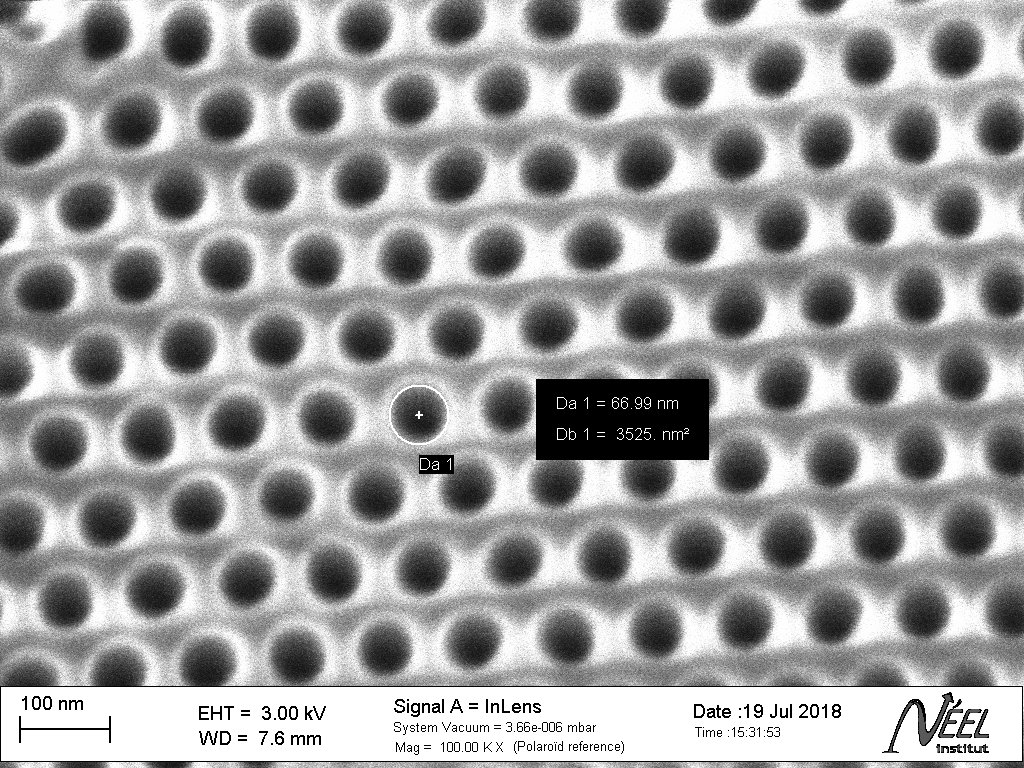
\includegraphics[width=0.9\textwidth]{images/296g_sol_side.jpg}
      \label{fig:295g-sol-side}}
      \\
      \subfloat[]{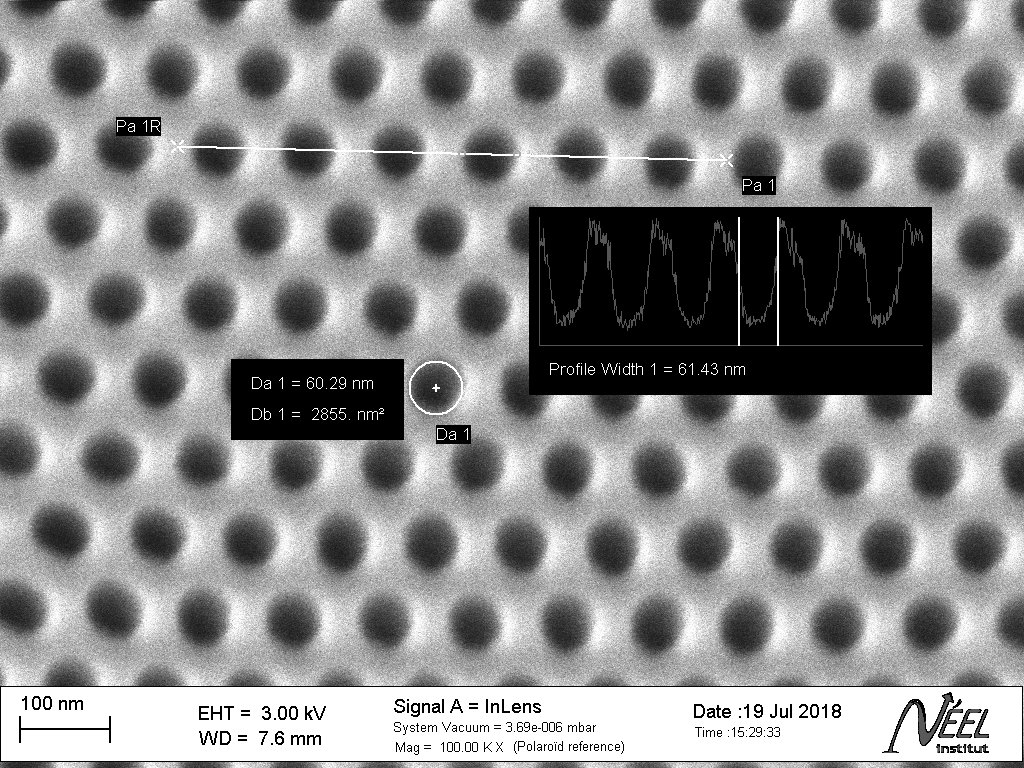
\includegraphics[width=0.9\textwidth]{images/296g_al_side.jpg}
      \label{fig:295g-al-side}}
      \caption{Electron beam microscopy images of membrane 295g' with measurements of the pore diameters on the solution side \protect\subref{fig:295g-sol-side} and aluminum side \protect\subref{fig:295g-al-side}.}
      \label{fig:meb-funnelling}
    \end{figure}

    All in all, it is hard to draw a conclusion on wheather thinner membranes do really improve things. For open pore membranes, the results hint at a decrease of the funnellization aspect, while for the closed pore membranes no such behaviour is observable. Even though the open pore $l_\mathrm{pore}=\SI{30}{\micro\meter}$ membranes yield the steepest isotherms we have recorded so far, it cannot be excluded that the pores show less defects simply by chance. For further confirmation, that it is really the thinner membranes and the long floating upon the \textit{barrier layer} dissolution process that make for these isotherm shapes, another wafer needs to be produced and measured in the same way as wafer 295.


  \section{Pore size reduction using atomic layer deposition}
  \label{sec:ald-experiments}

    Since the open pore membranes of wafer 295 proved to produce very steep isotherms, the goal of sub ten nanometer pore diameters is targeted. The idea is to reduce the pore diameters by atomic layer deposition (ALD) (compare \cref{subsec:ald}). As a reminder, \cref{fig:w295-processing-plan} shows the treatments and measurements of the inspected membranes of wafer 295.

    \subfile{tikz/graphs/295e_ALD/295e_ALD.tex}


    \subsection{Atomic layer deposition effectively reduces pore diameters}
    \label{subsec:ald-reduces-diameters}

      The first important question is: Does ALD work to reduce the pore diameters at all? To answer this, membrane 295e' has been deposited with 100 cycles of ALD and then measured in the experimental setup. In addition to that, SEM images have been recorded. The measurement results are shown in \cref{fig:295e-ald}. While the result for the first 100 cycles of ALD matches expectations perfectly, the second 100 cycles give a very different impression. The detailed discussion of the isotherm of membrane 295e''' shall be postponed in favor of the analysis of 295e' and 295e'' at this point.

      Firstly, the shape of the volumetric isotherm does not change for membrane 295e'' in comparison to 295e'. It is only shifted towards lower pressures. The hysteresis increases by a little bit which can be explained by the logarithmic context of realtive pressure to pore diameters though. Regarding the isotherms of 295e' and 295e'' on a \textsc{Kelvin} diameter axis as shown in \cref{fig:295e-ald-kelvin}, the change of the hysteresis disappears and the evaporation branches show the same steepness for both membranes. Furthermore, the diameter reduction by 100 cycles of ALD according to the isotherms is
      \begin{equation*}
        \Delta d_\mathrm{pore}^\mathrm{295e'\rightarrow 295e''}=\SI{20}{\nano\meter}
      \end{equation*}
      which makes for
      \begin{equation*}
        \delta d_\mathrm{pore}^\mathrm{exp} =\SI{2}{\angstrom}
      \end{equation*}
      diameter reduction per ALD cycle. This value is not far from the expectations of
      \begin{equation*}
        \delta d_\mathrm{pore}^\mathrm{theo} = \SI{2,2}{\nano\meter}
      \end{equation*}
      per cycle (compare \cref{subsec:ald}).

      The tranmission measurements also yield very sharp drops for the membranes 295e' and 295''.


    \subsection{Diameter reduction by atomic layer deposition is reproducible}
    \label{subsec:diameter-reduction-reproducible}

      Next, membrane 295e''' and 295f'' must be compared to probe the reproducibility of the pore diameter reduction using ALD. On the one hand, the membranes 295e' and 295f' yielded equivalent measurement results (please refer to \cref{fig:295-op}) and on the other hand both, 295e''' and 295f'', have undergone 200 cycles of ALD in total. So the two membranes' measurements should produce similar results.

      The measured data is plotted in \cref{fig:295-e-f-ald}. While the overall picture of the two membranes seems to match, clearly there is a shift towards lower pressures visible for membrane 295f''. Anyways, the membranes used for this comparison both show isotherms that do not match expectations and imply that the ALD did not work out properly. According to \cref{subsec:ald-reduces-diameters}, it works for only 100 cycles and also, the result seems independent of the ALD process being interrupted during the full 200 cycles. This leads to the conclusion that something is off for smaller diameters. Further analysis will follow in the upcoming section.

      Talking reproducibility, a tendency towards yes is justifiable but needs to be confirmed through further experiments.

      \subfile{tikz/graphs/295_e_f_ALD/295_e_f_ALD.tex}


      \subsection{Atomic layer deposition parameters need improvement}
      \label{parameters-need-improvement}

        \subfile{tikz/graphs/295_e_f_ALD/295e_200ALD.tex}

        In the following, the transition from membrane 295e'' to 295e''' using 100 layers of ALD shall be analysed. \Cref{fig:295-e-200ald} shows the measured isotherms on a relative pressure axis. The condensation in two steps together with a one step evaporation hints at a population of closed pores or open pores with constricted openings. Therefore, the isotherms are plotted on a \textsc{Kelvin} diameter axis in \cref{fig:295-e-200ald-kelvin} twice, once using the conversion for open pores (\cref{eq:p-sp}) and once that closed pores (\cref{eq:p-eq}). A black circle marks where the two steps of the isotherm's condensation branch superimpose on the same diameter range as a result. Moreover, another circle marks the corresponding transmission drops. They are both shifted towards higher pore diameters in comparison to the volumetric signals of condensation. Still, the two are aligned on the same diameter range. These observations back the suspicion of closed or constricted pores.
        \medskip

        \subfile{tikz/graphs/295_e_f_ALD/295f_200ALD.tex}

        \begin{figure}[p]
          \centering
          \subfloat[]{
            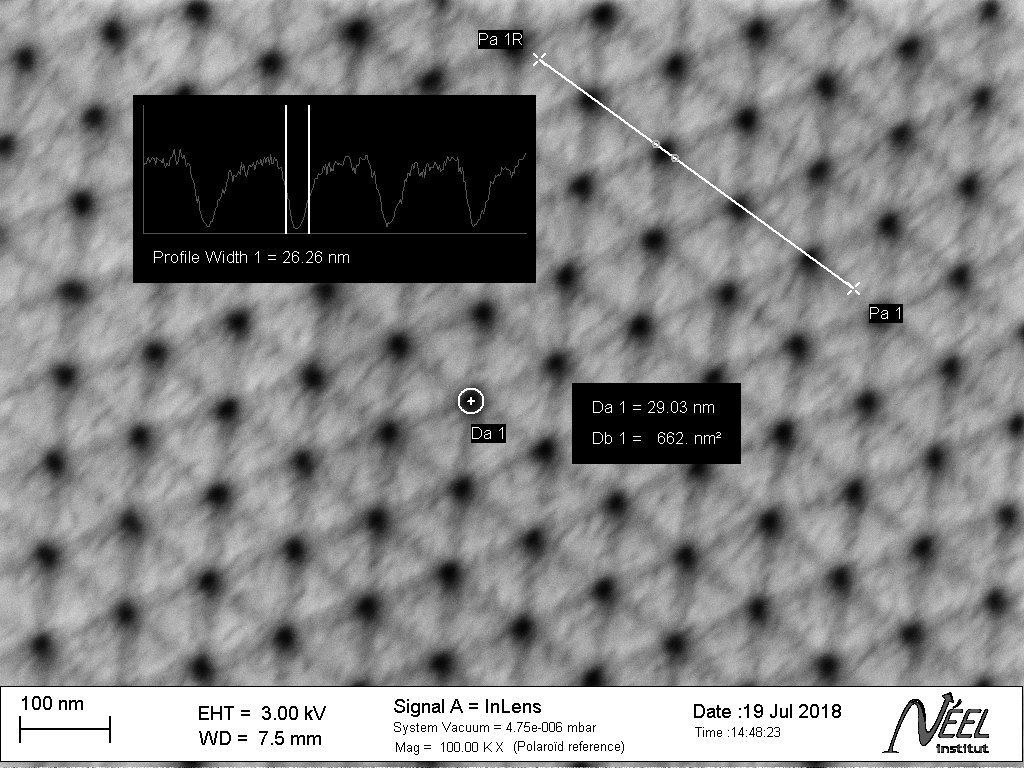
\includegraphics[width=0.9\textwidth]{images/295f_200ALD_sol_side.jpg}
            \label{fig:295f-200ald-sol-side}
          }
          \\
          \subfloat[]{
            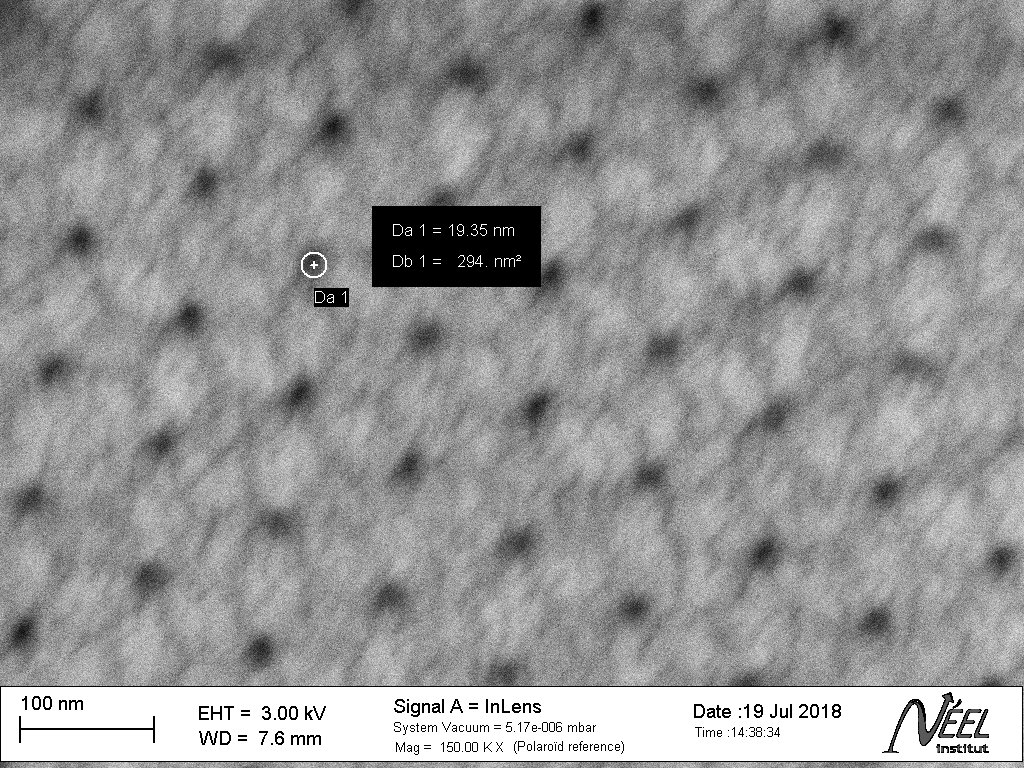
\includegraphics[width=0.9\textwidth]{images/295f_200ALD_al_side.jpg}
            \label{fig:295f-200ald-al-side}
          }
          \caption{Electron beam microscopy images of membrane 295f'''. \protect\subref{fig:295f-200ald-sol-side} and \protect\subref{fig:295f-200ald-al-side} show images of the solution and aluminum side with pore diameter measurements.}
          \label{fig:295f-200ALD-sem}
        \end{figure}

        Already in \cref{subsec:diameter-reduction-reproducible}, the similarity between the results of the membranes 295e''' and 295f'' has been analysed. For the sake of completeness, the same analysis as for membrane 295e''' shall be done for membrane 295f'' here. Again, the two step condensation together with the single step evaporation hint at closed or constriced pores. Using the \textsc{Kelvin} equations (\cref{sec:kelvin-equation}) to convert the relative pressure to diameters for closed and open pores yields the same superposition as observed for membrane 295e''' (marked by black circles for volumetrics and transmission). In addition to the volumetric and the transmission measurements, for membrane 295f'' SEM images have been recorded. \Cref{fig:295f-200ald-sol-side} and \cref{fig:295f-200ald-al-side} show the solution and aluminum side of the membrane. The pore diameters of
        \begin{equation}
          \begin{split}
              d_\mathrm{pore,SEM}^\mathrm{295f'',Sol}=\SI{29}{\nano\meter}, \\
              d_\mathrm{pore,SEM}^\mathrm{295f'',Al}=\SI{19}{\nano\meter}
          \end{split}
        \end{equation}
        approximately match the diameters derived from the condensation branches of the volumetric isotherms, whereas the evaporation branch would imply pore diameters of about
        \begin{equation}
          d_\mathrm{pore,evap}^\mathrm{295d''}=\SI{10}{\nano\meter}.
        \end{equation}
        Up to this point though, the evaporation branch has been assumed to be more precise for measuring the pore diameters as it only depends on equilibrium pressure.
        \medskip

        Finally, \cref{fig:295d-200ALD} shows the isotherm data of membrane 295d''. While there is still a volumetric signal visible, its pressurewise position does not match expectations as the deposit of 250 layers should make for smaller pores than the 200 layer on the membranes 295e''' and 295f''. Therefore, the signal might very well be due to noise of the measurements. On the other hand, also the transmission signal shows a drop. The signal does not rise again even at saturated vapor pressure though. This observation implies blocked pores that do not fill at all.

        \subfile{tikz/graphs/295d_ALD/295d_250ALD.tex}
        \subfile{tikz/graphs/295c/295c.tex}
        \begin{figure}[p]
          \subfloat[]{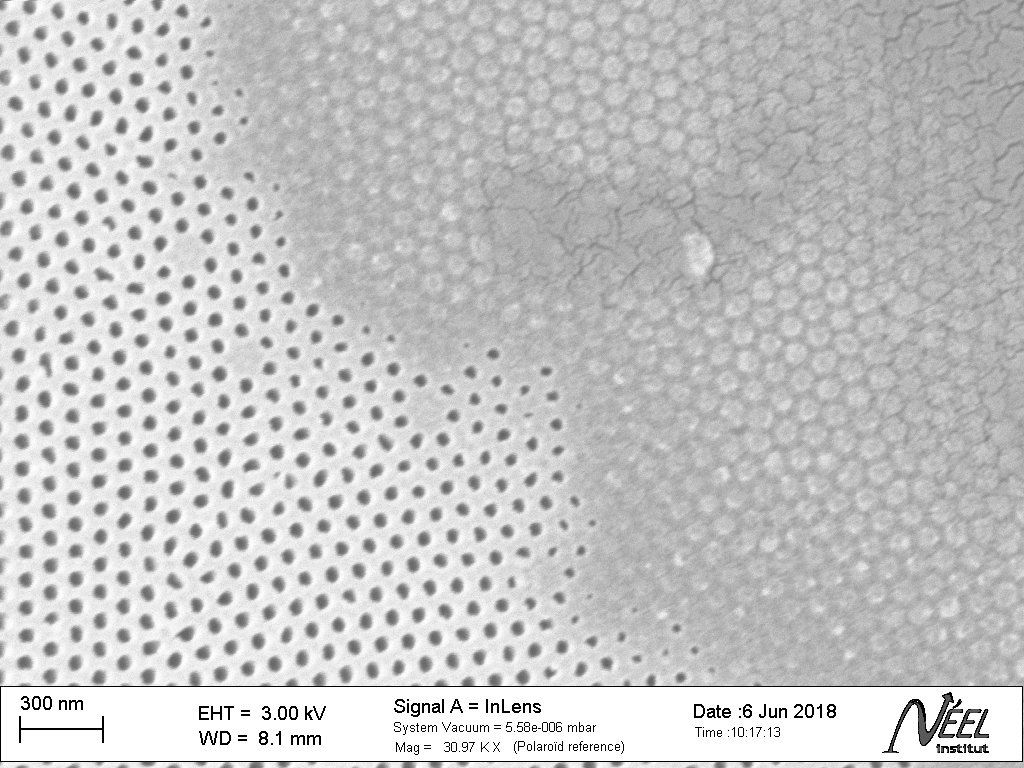
\includegraphics[width=0.9\textwidth]{images/295c_al.jpg}}
          \\
          \subfloat[]{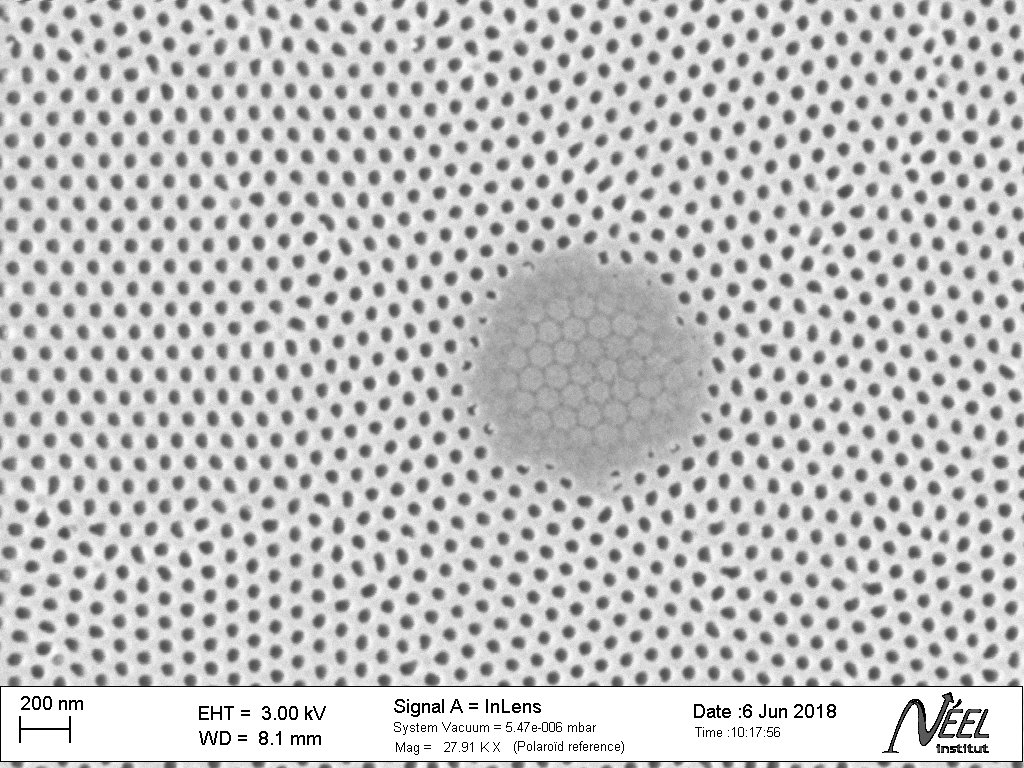
\includegraphics[width=0.9\textwidth]{images/295c_al_2.jpg}}
          \caption{MEB images of the aluminum side of membrane 295c. Areas of none open pores are clearly visible.}
          \label{fig:295c-meb}
        \end{figure}


          \section{Isotherms prove powerful to detect and characterize defects}
          \label{sec:theory-and-defects}


            Throughout the data evaluation, the volumetric measurements along with the laser transmission prove extremely sensitive to detect pore defect like closed pores, where they should be open, constrictions at the pore ends, corrugations or even funnellization. As a last example, membrane 295c' shall be analysed and the result applied to the other membranes of wafer 295.

            Expectations are that membrane 295c' shows the same properties as the other open pore membranes of wafer 295 as they were all floated on phosphoric acid still attached to the initial wafer except for 295b'. \Cref{fig:295c} displays its isotherm. In contrast to expectations, the isotherm shows a three step condensation branch while the evaporation branch consists of a single drop. An evaporation at high pressures that consists of a single sharp drop implies that all pores are distributed around a single diameter. As a consequence, the isotherm is plotted over pore diameters $d_\mathrm{pore}$ using \textsc{Kelvin} equation (\cref{sec:kelvin-equation}) for closed pores and open pores seperately and superimposed in one coordinate system (\cref{fig:295c-op-cp}). As the black circle tries to focus on, the first small rise at low pressures translates to the same pore diameter as the second one does for open pore analysis. This hints at a small population of closed pores on the wafer. In fact, the MEB images of the aluminum side of membrane 295c shown in \cref{fig:295c-meb} actually do show areas of none open pores which fill at equilibrium pressure which is coherent with the before made assumptions based on the volumetric isotherms. Moreover, regarding the laser transmission signal, another phenomenom implying pores filling at equilibrium pressure an be found. As amplified in \cref{fig:295c}, the transmission drops at about the same pressure as the first liquid fraction rise finishes and stays at this lower value until the occurence of the spinodal condensation where it drops farther. This drop can be explained by some pores filling and scattering light (compare \cref{sec:scattering-in-alumina-membranes}).

            As for the third rise of the volumetric isotherm's condensation branch, it can be explained by pore size distribution of open pores with two peaks. As there is no known reason for this kind of distribution, this explanations seems unlikely though. At this point, no other interpretation has been concluded with.


    \section{Unsolved transmission observations}
    \label{sec:unsolved-transmission}

              \subfile{tikz/graphs/292_295_296_transmission/292_295_296_transmission.tex}

              Firstly, a completely filled membrane should always yield a higher transmission coefficient $T$ than it would in its dry state according to the theory of index matching as explained in \cref{sec:scattering-in-alumina-membranes}. This fact serves as a tool to optically detect membranes that do not fill completely due to constrictions which by experience show a weaker tranmission after the condensation process is complete than they did before. Furthermore, due to the disorder created by pore filling and emptying, the transmission drops during the processes. Phenomena occurring on the volumetric measurements can therefore be linked to the measured transmission coefficient.

              Moreover, the phenomenom of the transmission dropping to lower values for the condensation than for evaporation branch of a given isotherm has been repeatedly observed on open pore membranes. An example is given by membrane 292d's isotherm, which is displayed in \cref{fig:292-trans}. At this point it must be mentioned that all open pore membranes measured before the wafers 295 and 296 have shown this same transmission characteristics. As interpretation serves the degree of disorder caused inside the membrane by the respective process. As the membrane contains pores open on both ends, the condensation occurs at spinodal pressure $P_\mathrm{sp}(d_\mathrm{pore})$. Due to the distribution of pore sizes, funnelization, corrugation and constrictions, the pores fill at different pressures $P_\mathrm{sp}^1 \neq P_\mathrm{sp}^2$. At a given pressure
              \begin{equation*}
                  P_\mathrm{sp}^1 < P < P_\mathrm{sp}^2,
              \end{equation*}
              where $P_\mathrm{sp}^1$ shall correspond to the smallest pore diameter found on the membrane and $P_\mathrm{sp}^2$ the largest one, the state of the me{}mbrane regarding filled and empty pores is assumed to be comparable to figure \cref{fig:disorder-absorption}. The hexane evaporates at equilibrium pressure $P_\mathrm{eq}$, though. That means that, assuming the same pore size distribution, funnelization, corregation and constrictions, the pores empty continuously. The theoretical state of the membrane is visualized in \cref{fig:disorder-desorption}.

              The difference is given by the most significant contrasts between neighboring pores during the condensation process, in explanation empty and filled pores, for spinodal condensation, while for evaporation at equilibrium pressure the pores only show different levels of liquid during most of the process. As a result, the absorption of hexane creates a higher grade of disorder than the desorption and therefore causes a more significant drop of the transmission coefficient (compare \cref{fig:292-trans}).
              \medskip

              The splitting of the evaporation drop into two dips seperated by a small local maximum cannot be explained by this theory, nor by any other means mentioned in this report. Moreover, the later analysed membranes of wafer 295 and 296 yield a more even dip distribution (compare \cref{fig:295-trans} and \cref{fig:296-trans}) and upon reducing the pore diameter of 295 using ALD, the membranes even show the inverse behaviour (\cref{fig:295f200ALD-trans}).

              In connection with the sharper isotherms, the first phenomenom could be explained by the pores being less flawed talking corrugations and funneling. The latter assumption is backed by the fact, that the transmission drops of 295d are of smaller magnitude than those of 296b. While both are open pore membranes, membrane 295d is only half as thick as 296b meaning that the pores are only half as long and therefore, the influence of the funnellization is reduced as has been explained in \cref{sec:thinner-membranes}.

              The second phenomenom of the deeper evaporation dip remains unclear though.

              \subfile{tikz/transmission_disorder/pore_disorder.tex}


  \section{Conclusions and prospects}

    The experiment setup measures reproducible isotherms for nanoporous alumina membranes. Currently, the experiment setup using helium as a fluid is put into operation.

    For the membrane production, the inhomogeneity of one single wafer has been concluded. These dispersions appear on the isotherms of closed pore membranes already. It remains to be probed if the inhomogeneities only origin from the anodization or also from the aluminum dissolution process, since the latter has been proven to cause changes to the pores in \cref{sssec:al-diss-bath} The pore opening step does not seem to increase the dispersion of the pores as the isotherms are more steep than before pore opening. On the contrary, it seems to improve things by decreasing the funnellization as explained in \cref{subsec:inverse-funnelling}.

    The experiments on the \textit{barrier layer} dissolution process revealed the dispersion of the \textit{barrier layer} thickness between different wafer. Furthermore, the etch rate of phosphoric acid on the alumina membranes has been concluded to be nonisotropic (compare \cref{subsec:etch-rate}).

    Moreover, the reduction of the wafers' thickness resulted in open pore membranes that produce very steep volumetric isotherms with sharp transmission drops of a gaussian shape.

    These membranes were used to test the atomic layer deposition as a means to reduce the pore diameter. The conducted experiments showed that the technique does indeed work for large ($>\SI{40}{\nano\meter}$) pore diameters, whereas pore defects appear when approaching smaller pore diameters - at least for the parameters used by Laurent Cagnon. Hopes are, that longer exposure times in the ALD cycle will solve the problem.

    Regarding the condensation and evaporation models introduced in \cref{eq:cond-evap-non-ideal-pore}, my measurements confirmed the the model of condensation at spinodal pressure $P_\mathrm{sp}>P_\mathrm{eq}$ for open pores that yields a hysteresis.
    \medskip

    As explained in \cref{sec:unsolved-transmission}, the behaviour of the tranmission signal is not well understood. For more clarity, some experiments need to be repeated.  For instance, another $\SI{30}{\micro\meter}$ thick wafer must be produced to conclude if the thickness is the parameter making for not only the extremely steep volumetric isotherms, but also for the gaussian shape of the transmission drops.
    \medskip


    As the membranes of wafer 295 produce very steep isotherms, a first comparison of the diameter extracted from the volumetric isotherm using the \textsc{Kelvin} equations (or other more sophisticated models) and the one derived from the SEM images in a statistical way can and should be attempted. For the latter, the knowledge of the porosity can be used to set manual threshholds for the image binarisation under the assumption of a constant funnellization angle.





\end{document}
